%*******************************************************************************
% Copyright (c) 2014 Formal Mind GmbH and others
% All rights reserved. This program and the accompanying materials
% are made available under the terms of the Eclipse Public License v1.0
% which accompanies this distribution, and is available at
% http://www.eclipse.org/legal/epl-v10.html
% 
% Contributors:
%     Michael Jastram - initial Copy
%     Maha Jastram - susequent improvements
%******************************************************************************/

We hope you find this reference manual useful.  It's a work in progress and will be actively improved and expanded.

% ===================================================================================
\section{Editors}
% ===================================================================================

\begin{wrapfigure}{l}{.3\linewidth}
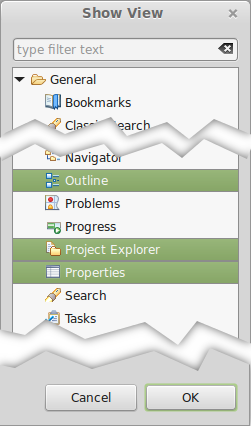
\includegraphics[height=.9\textwidth]{../rmf-images/views_highlighted.png}
\caption[flushleft]{Views.}
\label{fig:Views}
\end{wrapfigure}

Upon opening a ReqIF Model, the editor opens providing an overview of the model.  In essence what you are seeing is the Eclipse Workbench, with several modifications.  Here you will find a quick overview of each component.  A more detailed description of the Workbench can be found in Eclipse's Workbench User Guide.

A model contains any number of specifications, and the details of each specification can be inspected individually.  The windows in which all relevant information appears are called Views.  At your disposal are many Views with productivity, debugging, help and team resources.  We will be focusing only on the Views relevant to ProR.

% ===================================================================================
\subsection{ReqIF Overview Editor}
% ===================================================================================

This figure was briefly described in the tutorial.  Here we'll go deeper in depth.

\begin{figure}[h!]
  \centering
  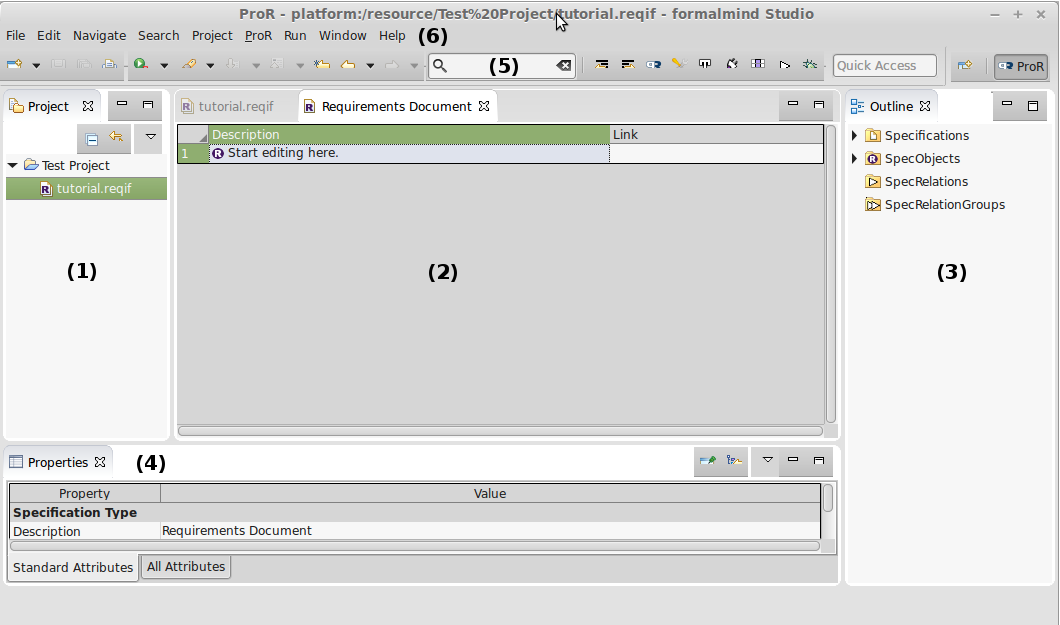
\includegraphics[width=\linewidth]{../rmf-images/Screenshot_intro.png}
  \caption{The \pror{} user interface}
  \label{fig:user_interface_overview}
\end{figure}

(1) is the Project Explorer window.  Here you will see a hierarchical listing of the project and the associated models.

(2) The Editor shows you a hierarchical breakdown of the model.  Each specification with it's associated SpecObjects is listed in a spreadsheet.  Because the SpecObjects of each requirement can vary, not all fields will be completed.  Because the fields need to  be created and then associated with the SpecObjects, they may not all be (nor do they need to be) represented.  But what appears and how they appear can be customized.

In the Editor, you see the SpecObjects that exist in this Specification.
There is currently only one, with the description "Start editing here".

The Outline (3) has four folders:

\begin{itemize}

\item
  "Specifications" shows the Specifications in the ReqIF.  You can
  expand the tree to expose the hierarchy of SpecObjects in the
  ReqIF model.
\item
  "SpecObjects" shows all SpecObjects in the ReqIF model as a flat list.
  Keep in mind that SpecObjects in Specifications are references.  In
  contrast, this folder shows all SpecObjects created for the ReqIF model, whether or not they are referenced.
\item
  "SpecRelations" shows all SpecRelations in the ReqIF as a flat list.
  For now, we will ignore SpecRelations.
\item
  "SpecRelationsGroups" represent an optional mechanism for grouping SpecRelations between two specific Specifications.
\end{itemize}

The properties of a selected Element are shown in the Properties view
(4).  As the only Requirement in the model is selected, we see its
SpecObjectType ("Requirements Type") and its only Attribute
("Description") with the value "Start editing here.".  There are two
tabs "Standard Attributes" and "All Attributes" at the bottom of the
Properties view.  ***** The "Standard Attributes" tab shows you all standard
attributes of the selected element.  The "All Attributes" shows all
existing ReqIF attributes of the selected element.

Above the main working windows it the tool bar (5) and, at the very top, the menu bar (6).
\subsection{Specification Editor}

% ===================================================================================
\section{Views}
% ===================================================================================

By default, ProR's Workbench displays the following three views:

% -----------------------------------------------------------------------------------
\subsection{Project Explorer View}\index{Project Explorer View}
% -----------------------------------------------------------------------------------

% -----------------------------------------------------------------------------------
\subsection{Properties View}\index{Properties View}
% -----------------------------------------------------------------------------------

% -----------------------------------------------------------------------------------
\subsection{Outline View}\index{Outline View}
% -----------------------------------------------------------------------------------

% ===================================================================================
\section{Configurations}
% ===================================================================================


The ProR menu contains entries to launch a number of configuration
dialogs.

% -----------------------------------------------------------------------------------
\subsection{General Configuration}
\index{Configuration!General}
% -----------------------------------------------------------------------------------

% -----------------------------------------------------------------------------------
\subsection{Datatype Configuration}
\index{Configuration!Datatype}
% -----------------------------------------------------------------------------------

This configuration is opened via ProR \textbar{} Datatype Configuration
...

The dialog shows two folders, one for SpecTypes and one for Datatypes.
SpecTypes are created for typing elements that have attributes
(SpecObjects, Specifications, SpecRelations).  New SpecTypes can be
created by right-clicking on the folder and selecting ``New Child''.
Through the same mechanism, attribute definitions can be added to a
SpecType.  attribute definitions are typed.  Selecting an element shows
its properties in the lower pane, where it can be configured.

Attribute definitions must have a name and a datatype.  Some attribute
definitions allow further customization.  The datatype is selected from a
dropdown.  New datatypes can be created by right-clicking on the folder
``Datatypes'' and selecting ``New Child''.  Again, selecting a datatype
shows its properties in the lower pane, where it can be configured.  A
datatype should have at least a long name.

As an example, consider the following Datatype Configuration Dialog:

\begin{figure}[h!]
\centering     
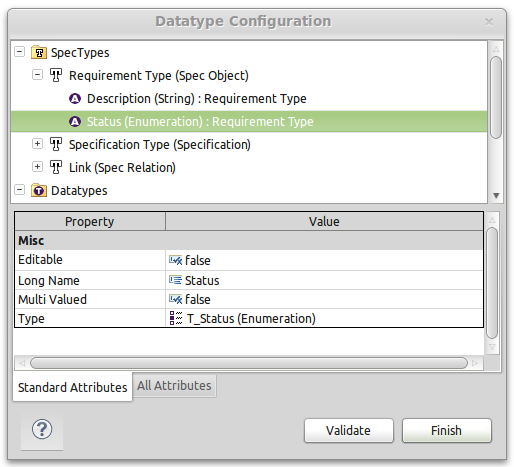
\includegraphics[width=0.8\linewidth]{../rmf-images/pror_datatype_configuration.png}
\caption{Datatype Configuration Dialog}      
\label{fig:DatatypeConfig}
\end{figure}

The Spec Type for ``Requirements Type'', which is applicable to
SpecObjects, is expanded.  The Spec Type has two attributes,
``Description'' (String) and ``Status'' (Enumeration).  Status is
selected, and in the pane below the mandatory values, ``Long Name'' and
``Type'' have been set.  Further customization of the attribute is
possible, e.g.  by converting it in a Multi-Valued attribute by setting
the corresponding flag to ``true''.

\subsubsection{Enumeration Datatypes}

An enumeration datatype must have enumeration values.  These are created
by right-clicking the enumeration datatype and selecting New Child
\textbar{} Enum Value.  You may have to unfold the enum value to select
it, so that you can provide it with a Long Name.  The following shows a
correctly configured enumeration datatype:

\begin{figure}[h!]
\centering      
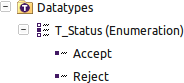
\includegraphics[width=0.4\linewidth]{../rmf-images/rmf_enumeration.png}
\caption{Enumerations}      
\label{fig:Enumerations}
\end{figure}

% -----------------------------------------------------------------------------------
\subsection{Presentation Configuration}\index{Configuration!Presentation}
% -----------------------------------------------------------------------------------

% -----------------------------------------------------------------------------------
\subsection{Column Configuration}\index{Configuration!Column}
% -----------------------------------------------------------------------------------

This configuration is specific to the Specification Editor.

The Column Configuration Dialog configures the Columns of a
Specification.  Columns are identified by name.  The width of the column
can be adjusted directly by dragging the column separator in the table
header.

If the SpecObject has an attribute where the name of the attribute
matches the name of the column, then that attribute is shown in that
column.
